\documentclass[letterpaper,12pt]{article}
\usepackage[margin=14mm,top=18mm,bottom=17mm,headheight=14pt]{geometry}
\pdfmapfile{+cm.map}\pdfmapfile{+cmextra.map}
\usepackage{tikz,fancyhdr,amsmath,amssymb}
\usetikzlibrary{arrows.meta,patterns}
\pagestyle{fancy}\fancyhf{}\renewcommand{\headrulewidth}{0pt}
\fancyhead[L]{\small Week 50 / Staircases and lengths / K--1}
\fancyfoot[L]{\small Bellingham Math Circle / Week 50 / F50-K-v2}
\fancyfoot[R]{\small\thepage}
\setlength{\parindent}{0pt}\setlength{\parskip}{0pt}
\begin{document}
\noindent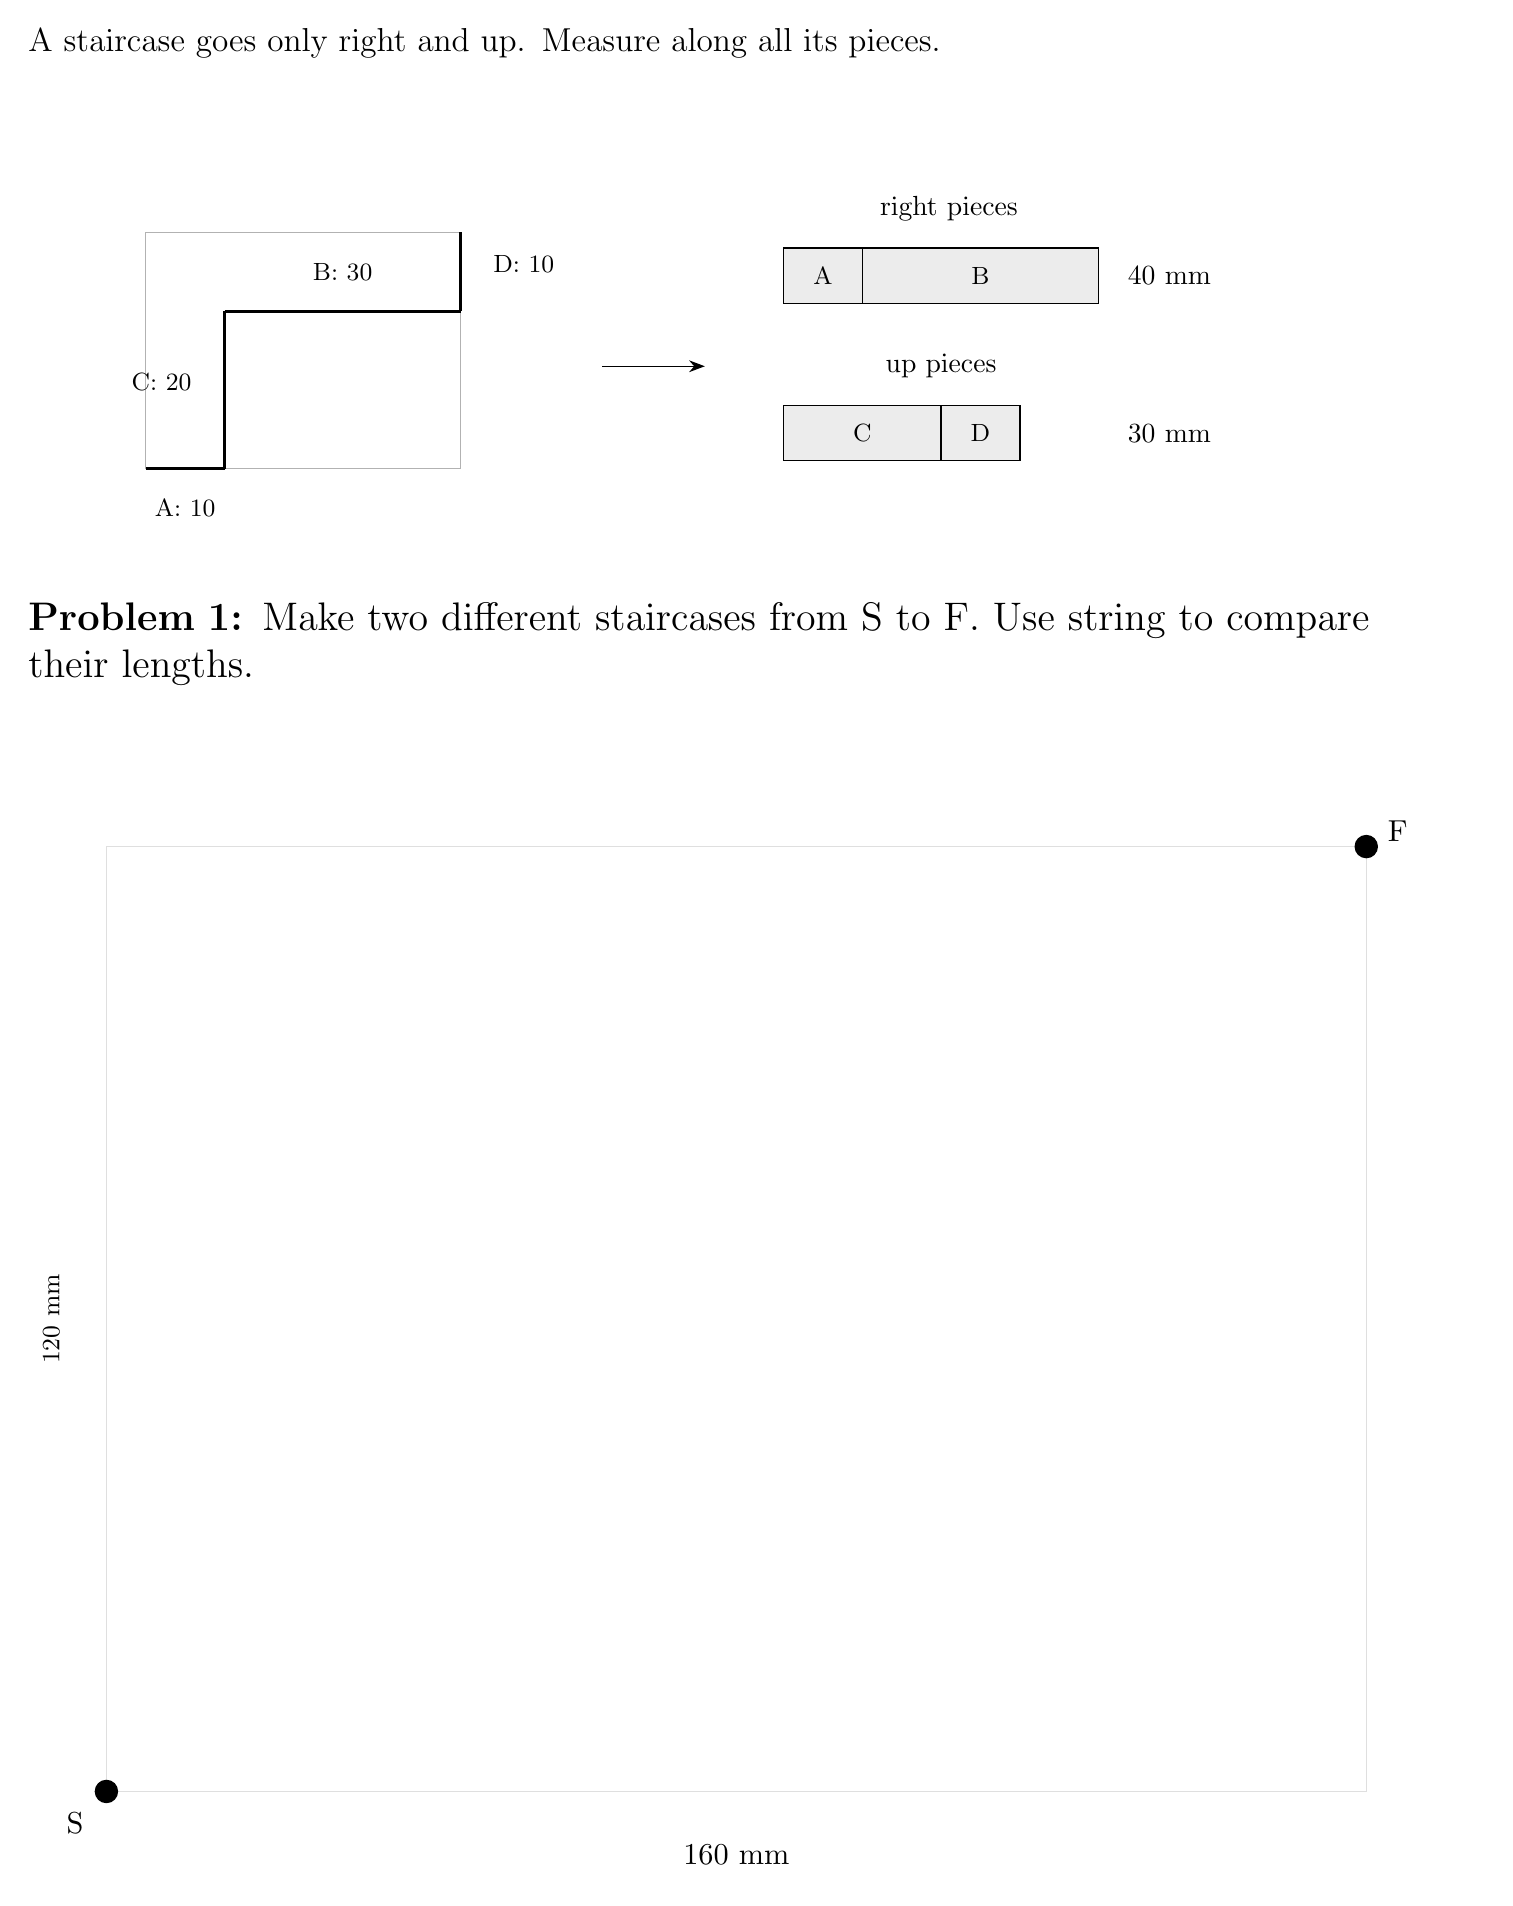
\begin{tikzpicture}[x=1mm,y=-1mm,line width=.5pt]
\path[use as bounding box] (0,0) rectangle (185,235);
\node[anchor=north west,inner sep=0pt,text width=180mm,font=\fontsize{12}{15}\selectfont] at (0,0) {A staircase goes only right and up. Measure along all its pieces.};
\draw[gray!60] (15,26) rectangle ++(40,30);
\draw[line width=1pt] (15,56) -- (25,56);
\draw[line width=1pt] (25,56) -- (25,36);
\draw[line width=1pt] (25,36) -- (55,36);
\draw[line width=1pt] (55,36) -- (55,26);
\node[anchor=center,inner sep=1pt,font=\fontsize{9}{11}\selectfont] at (20,61) {A: 10};
\node[anchor=center,inner sep=1pt,font=\fontsize{9}{11}\selectfont] at (17,45) {C: 20};
\node[anchor=center,inner sep=1pt,font=\fontsize{9}{11}\selectfont] at (40,31) {B: 30};
\node[anchor=center,inner sep=1pt,font=\fontsize{9}{11}\selectfont] at (63,30) {D: 10};
\draw[-{Stealth[length=2mm]}] (73,43) -- (86,43);
\draw[fill=gray!15] (96,28) rectangle ++(10,7);
\draw[fill=gray!15] (106,28) rectangle ++(30,7);
\node[anchor=center,inner sep=1pt,font=\fontsize{9}{11}\selectfont] at (101,31.5) {A};
\node[anchor=center,inner sep=1pt,font=\fontsize{9}{11}\selectfont] at (121,31.5) {B};
\node[anchor=center,inner sep=1pt,font=\fontsize{10}{12}\selectfont] at (145,31.5) {40 mm};
\draw[fill=gray!15] (96,48) rectangle ++(20,7);
\draw[fill=gray!15] (116,48) rectangle ++(10,7);
\node[anchor=center,inner sep=1pt,font=\fontsize{9}{11}\selectfont] at (106,51.5) {C};
\node[anchor=center,inner sep=1pt,font=\fontsize{9}{11}\selectfont] at (121,51.5) {D};
\node[anchor=center,inner sep=1pt,font=\fontsize{10}{12}\selectfont] at (145,51.5) {30 mm};
\node[anchor=center,inner sep=1pt,font=\fontsize{10}{12}\selectfont] at (117,23) {right pieces};
\node[anchor=center,inner sep=1pt,font=\fontsize{10}{12}\selectfont] at (116,43) {up pieces};
\node[anchor=north west,inner sep=0pt,text width=180mm,font=\fontsize{14}{17}\selectfont] at (0,73) {\textbf{Problem 1:} Make two different staircases from S to F. Use string to compare their lengths.};
\draw[gray!25,line width=.4pt] (10,104) rectangle ++(160,120);
\draw[fill=black] (10,224) circle (1.4);
\draw[fill=black] (170,104) circle (1.4);
\node[anchor=center,inner sep=1pt,font=\fontsize{11}{13}\selectfont] at (6,228) {S};
\node[anchor=center,inner sep=1pt,font=\fontsize{11}{13}\selectfont] at (174,102) {F};
\node[anchor=center,inner sep=1pt,font=\fontsize{11}{13}\selectfont] at (90,232) {160 mm};
\node[rotate=90,font=\small] at (3,164) {120 mm};
\end{tikzpicture}
\newpage
\noindent\begin{tikzpicture}[x=1mm,y=-1mm,line width=.5pt]
\path[use as bounding box] (0,0) rectangle (185,235);
\node[anchor=north west,inner sep=0pt,text width=180mm,font=\fontsize{14}{17}\selectfont] at (0,0) {\textbf{Problem 2:} Follow both staircases with string. Compare the two pieces of string.};
\draw[gray!25,line width=.4pt] (10,42) rectangle ++(160,120);
\draw[densely dotted,line width=.8pt] (10,162) -- (170,42);
\draw[line width=1.8pt] (10,162) -- (170.0,162.0) -- (170.0,42.0);
\draw[dashed,line width=1.4pt] (10,162) -- (10,102) -- (90,102) -- (90,42) -- (170,42);
\draw[fill=black] (10,162) circle (1.4);
\draw[fill=black] (170,42) circle (1.4);
\node[anchor=center,inner sep=1pt,font=\fontsize{11}{13}\selectfont] at (6,166) {S};
\node[anchor=center,inner sep=1pt,font=\fontsize{11}{13}\selectfont] at (174,40) {F};
\node[anchor=center,inner sep=1pt,font=\fontsize{11}{13}\selectfont] at (90,170) {160 mm};
\node[rotate=90,font=\small] at (3,102) {120 mm};
\node[anchor=north west,inner sep=0pt,text width=180mm,font=\fontsize{12}{15}\selectfont] at (9,184) {Circle: same length / solid longer / dashed longer};
\draw[line width=.7pt] (10,221) -- (110,221);
\draw[] (10,219) -- (10,223);
\draw[] (110,219) -- (110,223);
\node[anchor=center,inner sep=1pt,font=\fontsize{10}{12}\selectfont] at (60,227) {100 mm};
\end{tikzpicture}
\newpage
\noindent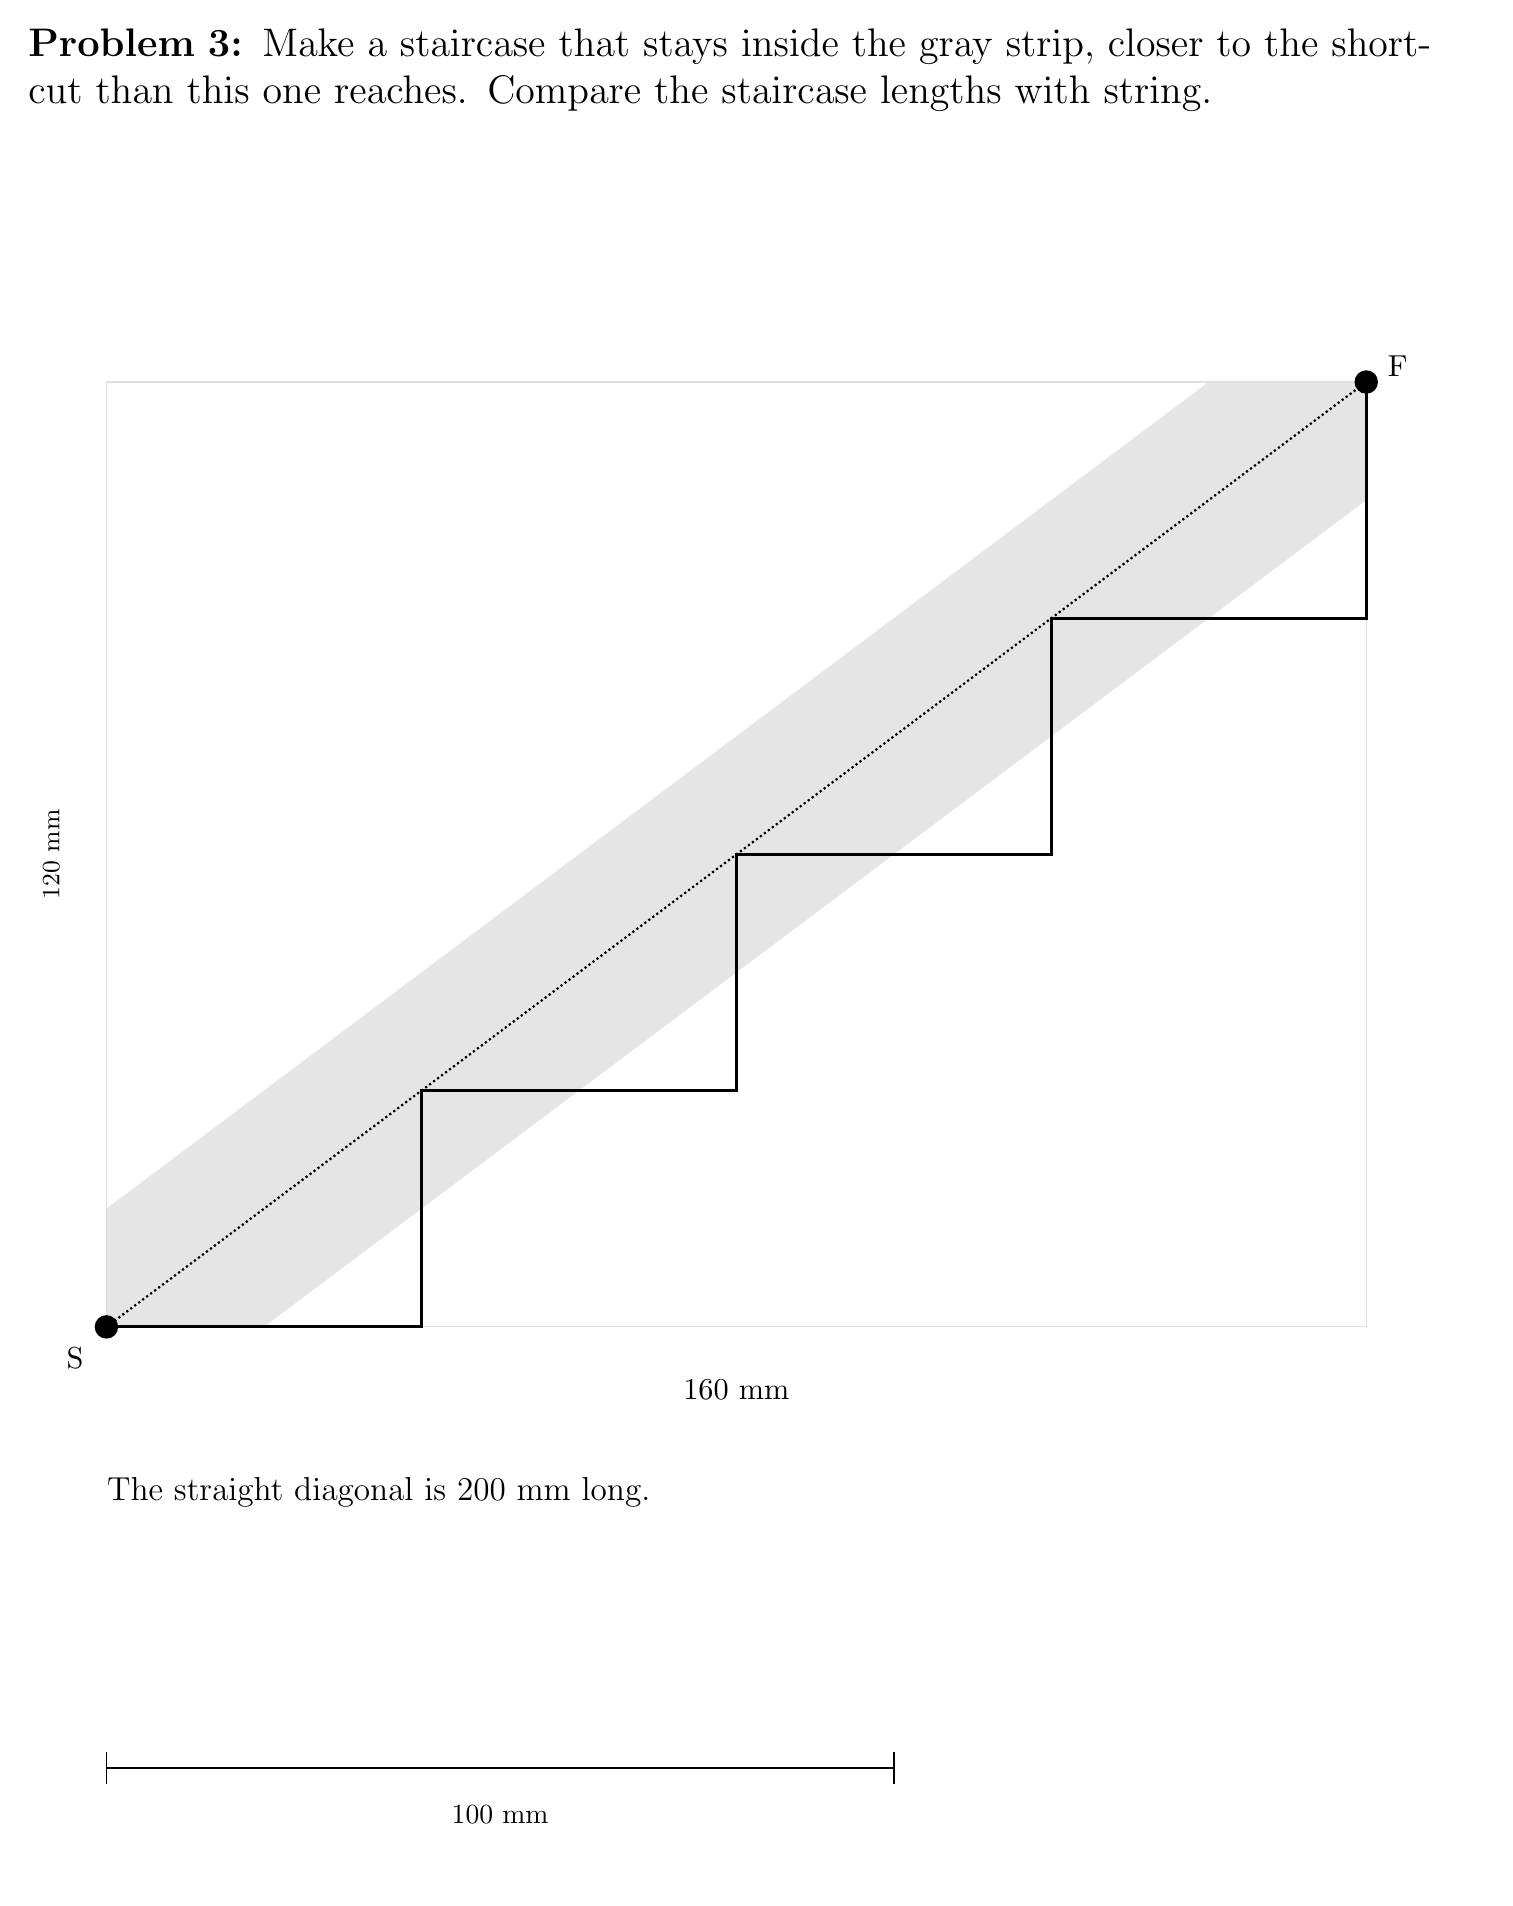
\begin{tikzpicture}[x=1mm,y=-1mm,line width=.5pt]
\path[use as bounding box] (0,0) rectangle (185,235);
\node[anchor=north west,inner sep=0pt,text width=180mm,font=\fontsize{14}{17}\selectfont] at (0,0) {\textbf{Problem 3:} Make a staircase that stays inside the gray strip, closer to the shortcut than this one reaches. Compare the staircase lengths with string.};
\fill[gray!20] (10,165) -- (10,150) -- (150.0,45) -- (170,45) -- (170,60) -- (30.0,165) -- cycle;
\draw[gray!25,line width=.4pt] (10,45) rectangle ++(160,120);
\draw[densely dotted,line width=.8pt] (10,165) -- (170,45);
\draw[line width=1.1pt] (10,165) -- (50.0,165.0) -- (50.0,135.0) -- (90.0,135.0) -- (90.0,105.0) -- (130.0,105.0) -- (130.0,75.0) -- (170.0,75.0) -- (170.0,45.0);
\draw[fill=black] (10,165) circle (1.4);
\draw[fill=black] (170,45) circle (1.4);
\node[anchor=center,inner sep=1pt,font=\fontsize{11}{13}\selectfont] at (6,169) {S};
\node[anchor=center,inner sep=1pt,font=\fontsize{11}{13}\selectfont] at (174,43) {F};
\node[anchor=center,inner sep=1pt,font=\fontsize{11}{13}\selectfont] at (90,173) {160 mm};
\node[rotate=90,font=\small] at (3,105) {120 mm};
\node[anchor=north west,inner sep=0pt,text width=174mm,font=\fontsize{12}{15}\selectfont] at (10,184) {The straight diagonal is 200 mm long.};
\draw[line width=.7pt] (10,221) -- (110,221);
\draw[] (10,219) -- (10,223);
\draw[] (110,219) -- (110,223);
\node[anchor=center,inner sep=1pt,font=\fontsize{10}{12}\selectfont] at (60,227) {100 mm};
\end{tikzpicture}
\newpage
\noindent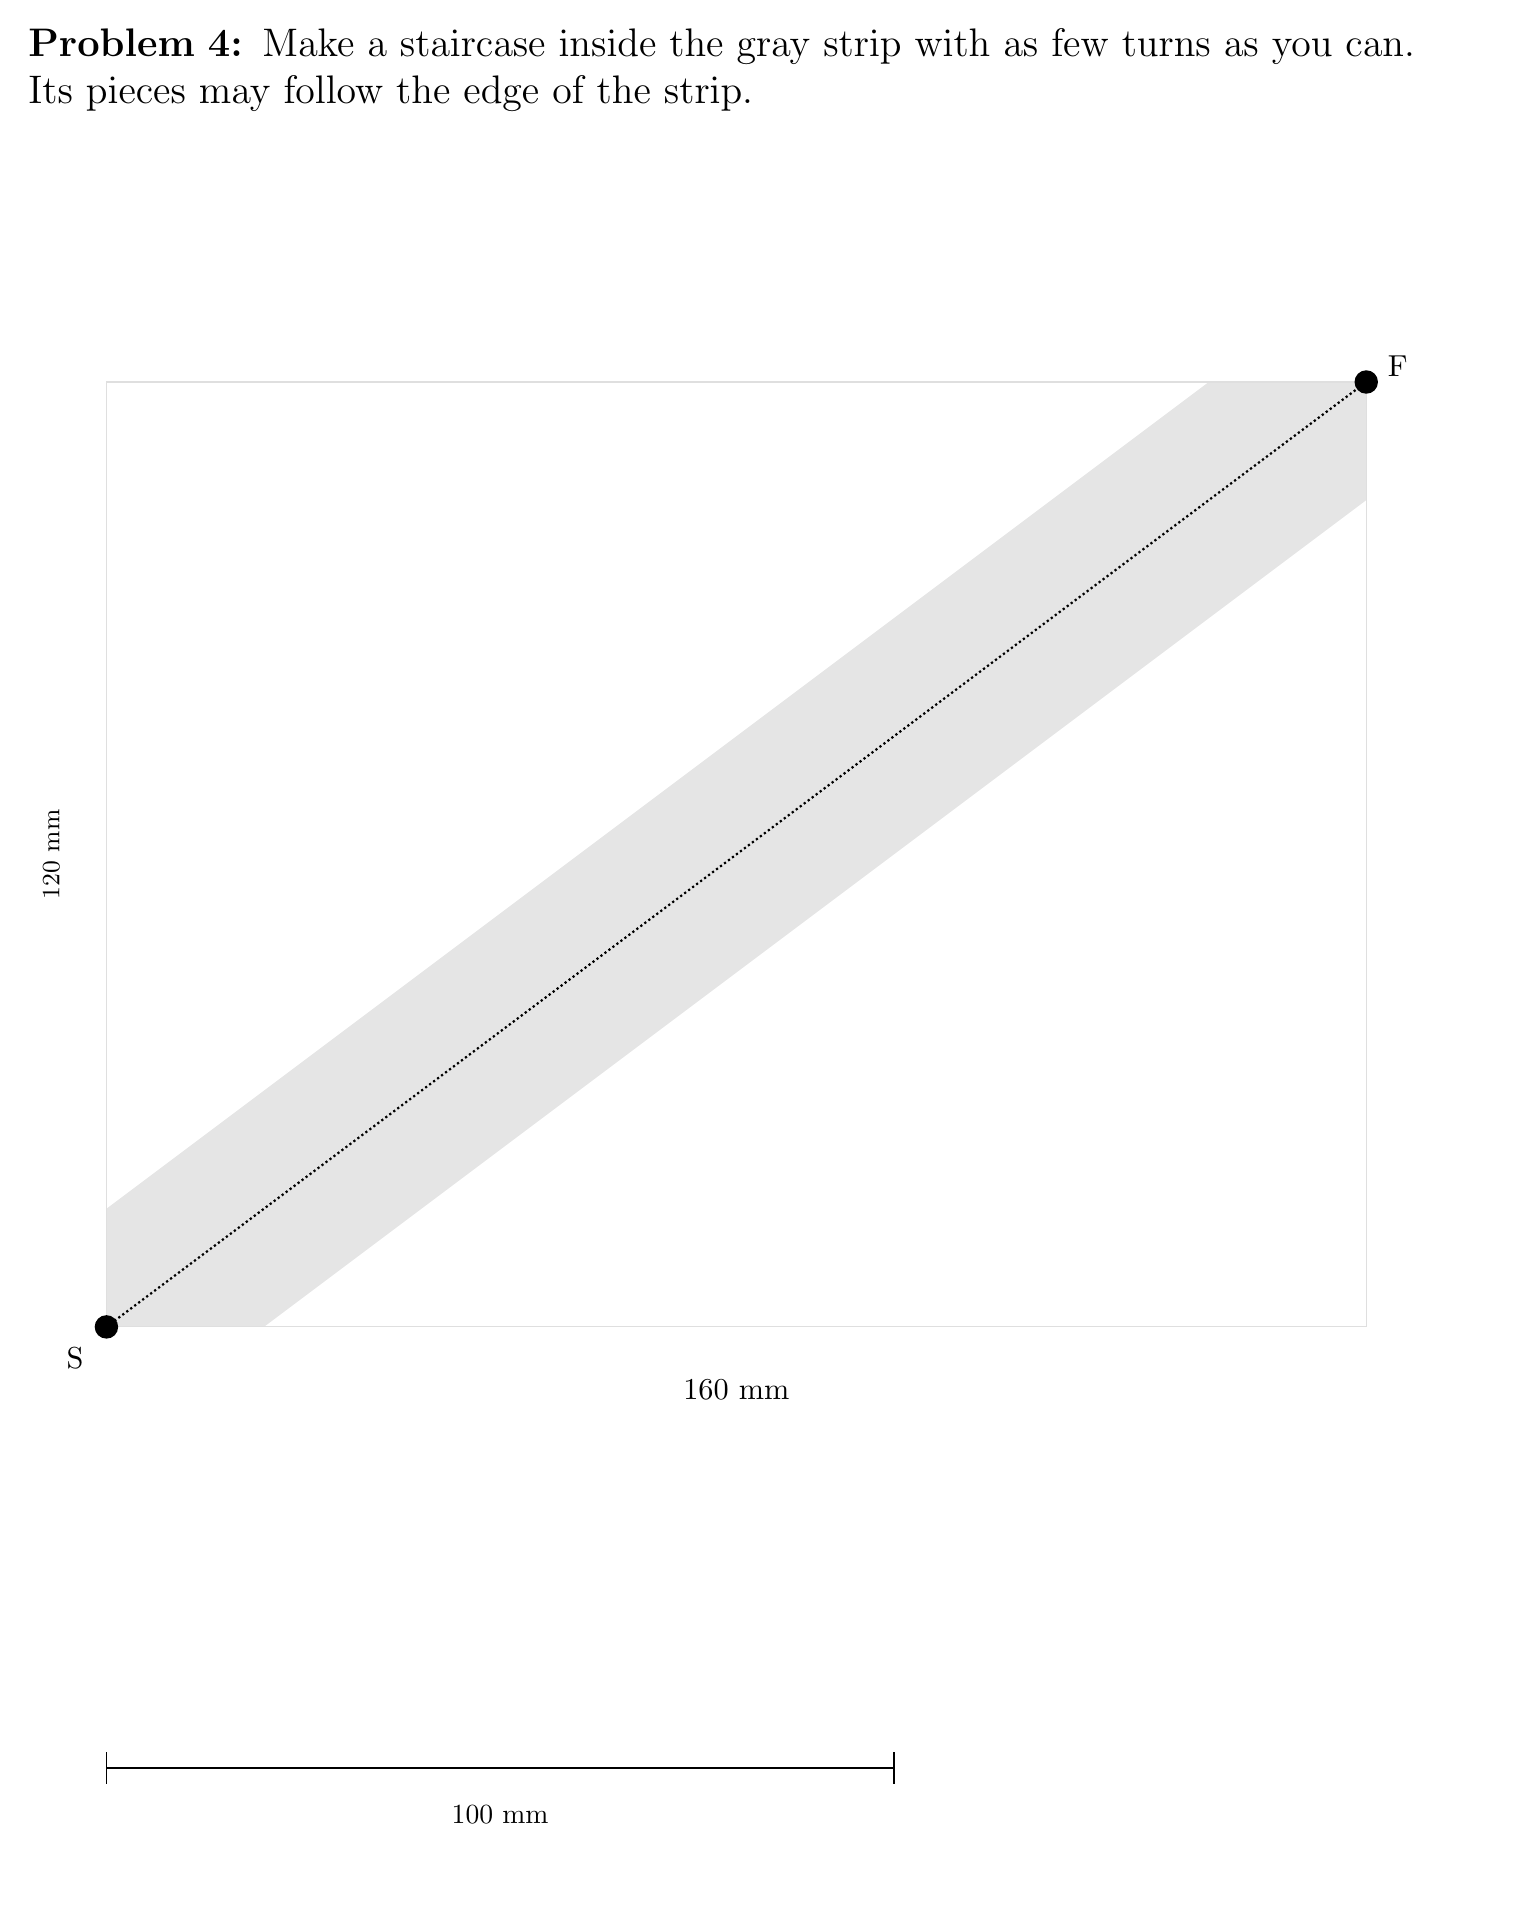
\begin{tikzpicture}[x=1mm,y=-1mm,line width=.5pt]
\path[use as bounding box] (0,0) rectangle (185,235);
\node[anchor=north west,inner sep=0pt,text width=180mm,font=\fontsize{14}{17}\selectfont] at (0,0) {\textbf{Problem 4:} Make a staircase inside the gray strip with as few turns as you can. Its pieces may follow the edge of the strip.};
\fill[gray!20] (10,165) -- (10,150) -- (150.0,45) -- (170,45) -- (170,60) -- (30.0,165) -- cycle;
\draw[gray!25,line width=.4pt] (10,45) rectangle ++(160,120);
\draw[densely dotted,line width=.8pt] (10,165) -- (170,45);
\draw[fill=black] (10,165) circle (1.4);
\draw[fill=black] (170,45) circle (1.4);
\node[anchor=center,inner sep=1pt,font=\fontsize{11}{13}\selectfont] at (6,169) {S};
\node[anchor=center,inner sep=1pt,font=\fontsize{11}{13}\selectfont] at (174,43) {F};
\node[anchor=center,inner sep=1pt,font=\fontsize{11}{13}\selectfont] at (90,173) {160 mm};
\node[rotate=90,font=\small] at (3,105) {120 mm};
\draw[line width=.7pt] (10,221) -- (110,221);
\draw[] (10,219) -- (10,223);
\draw[] (110,219) -- (110,223);
\node[anchor=center,inner sep=1pt,font=\fontsize{10}{12}\selectfont] at (60,227) {100 mm};
\end{tikzpicture}
\newpage
\noindent\begin{tikzpicture}[x=1mm,y=-1mm,line width=.5pt]
\path[use as bounding box] (0,0) rectangle (185,235);
\node[anchor=north west,inner sep=0pt,text width=180mm,font=\fontsize{14}{17}\selectfont] at (0,0) {\textbf{Problem 5:} A path may now go left as well as right and up. Make two different S-to-F paths that use the same amount of string and more than a staircase.};
\draw[gray!25,line width=.4pt] (10,40) rectangle ++(160,120);
\draw[densely dotted,line width=.8pt] (10,160) -- (170,40);
\draw[fill=black] (10,160) circle (1.4);
\draw[fill=black] (170,40) circle (1.4);
\node[anchor=center,inner sep=1pt,font=\fontsize{11}{13}\selectfont] at (6,164) {S};
\node[anchor=center,inner sep=1pt,font=\fontsize{11}{13}\selectfont] at (174,38) {F};
\node[anchor=center,inner sep=1pt,font=\fontsize{11}{13}\selectfont] at (90,168) {160 mm};
\node[rotate=90,font=\small] at (3,100) {120 mm};
\node[anchor=north west,inner sep=0pt,text width=180mm,font=\fontsize{14}{17}\selectfont] at (0,180) {\textbf{Problem 6:} Can a path with a leftward piece use less string than a staircase?};
\draw[line width=.7pt] (10,225) -- (110,225);
\draw[] (10,223) -- (10,227);
\draw[] (110,223) -- (110,227);
\node[anchor=center,inner sep=1pt,font=\fontsize{10}{12}\selectfont] at (60,231) {100 mm};
\end{tikzpicture}
\end{document}
